\chapter{Comparación sistemática}
\label{cap:comparacion}

Este capítulo responde a la RQ4: cómo pueden compararse las APIs de correo de forma sistemática para responder a preguntas de decisión que involucran simultáneamente requisitos funcionales y no funcionales.
La pregunta del ejemplo de la Sección~\ref{subsec:introduccion:ejemplo} es una de ellas.
Una aplicación necesita enviar 100.000 correos al mes, con ráfagas de 1.000 peticiones por minuto, \textit{webhooks} de eventos y envío en lote, y la pregunta es qué API y qué plan lo cubren al menor coste.
Para responderla hay que cruzar cuatro datos en cada una de las ocho APIs.
El precio con la cuota del plan, el caudal del \textit{endpoint} de envío y el tamaño máximo del lote están en la Datasheet, pero los \textit{webhooks} no, porque ACM2YAML v0.3 no modela funcionalidades.

El método que responde a preguntas como esta es la contribución C-04 (Sección~\ref{sec:introduccion:contribuciones}): un catálogo de preguntas de decisión propias del dominio y un procedimiento que las responde sobre las Datasheets.
Las preguntas de capacidad se calculan con PRIME4API, el motor de análisis de la capacidad de Gavira Sánchez \citep{gavira2026tfm}, y se contrastan con un cálculo a mano.
Las funcionales se leen en la matriz de \textit{features}, la tabla de funcionalidades por plan que acompaña a cada Datasheet.

El capítulo se organiza del siguiente modo.
En primer lugar, la Sección~\ref{sec:comparacion:catalogo} presenta las 32 preguntas del catálogo y la clase que dice con qué se responde cada una.
A continuación, la Sección~\ref{sec:comparacion:procedimiento} aplica el procedimiento a las ocho Datasheets y mide la cobertura, y la Sección~\ref{sec:comparacion:harvey} trata las cuatro preguntas que piden HARVEY4API.
Después, la Sección~\ref{sec:comparacion:caso} responde con el catálogo al caso de los 100.000 correos, y la Sección~\ref{sec:comparacion:funcional} compara las funcionalidades de cada plan.
Por último, la Sección~\ref{sec:comparacion:respuesta} responde a la RQ4.

\section{Catálogo de preguntas de decisión}\label{sec:comparacion:catalogo}\label{sec:hallazgos:catalogo-pi}

Una plantilla de pregunta es una pregunta con huecos, como la API, el plan, el volumen o el precio, que se rellenan para cada caso.
El catálogo tiene 32 plantillas, y 25 de ellas (el 78~\%) se pueden responder con el instrumental del canal API: la Datasheet, PRIME4API y HARVEY4API.
De esas 25, 11 se responden leyendo la Datasheet, 10 con una operación de PRIME4API y 4 con HARVEY4API.
Otras 2 se responden leyendo una matriz de \textit{features} por plan, que se captura con las mismas fuentes que la Datasheet pero queda fuera del esquema.
Las 5 restantes no tienen respuesta, y cada una deja escrito qué falta para tenerla.

La proporción de preguntas respondibles es la cobertura, la misma métrica con la que Cavero et al., que definen el Pricing Intelligence como disciplina, miden el alcance de sus herramientas: un 54~\% sobre un banco de 56 plantillas \citep{cavero2026pricingintelligence}.

Las dos cifras no se miden igual.
Cavero et al.\ prueban herramientas que ya existían contra un banco que no se hizo para ellas, y aquí la clase de cada pregunta, el instrumento con el que se responde, se asigna conociendo el instrumental.
La categoría B, la de selección de suscripción, parte de las operaciones del motor, y las cuatro preguntas que el catálogo asigna a HARVEY4API cuentan por la especificación de la herramienta, que no se ha ejecutado.
Sin esas cuatro, la cobertura con un instrumento leído o ejecutado es de 21 sobre 32, el 66~\%.

Del trabajo de Cavero et al.\ se toma también la gramática de las plantillas, con siete \textit{placeholders} (los huecos): la API (\texttt{SAAS}), el plan con sus complementos (\texttt{CONFIGURATION}), una funcionalidad (\texttt{FEATURE}), una cantidad como un volumen de correos o una ventana de tiempo (\texttt{USAGE LIMIT}), la necesidad del usuario (\texttt{ACTION}), un precio (\texttt{PRICE}) y el año de una versión del \textit{pricing} (\texttt{YEAR}).
Ninguna plantilla nombra una API, porque el proveedor solo aparece al rellenar los huecos, en el ejemplo de cada pregunta, y 13 de las 32 hablan de correo, como los envíos al mes o los límites que crecen con la reputación del remitente.
Con esa gramática, cada pregunta del catálogo puede incorporarse al banco de plantillas del grupo ISA de la Universidad de Sevilla.

Cada pregunta tiene una plantilla, un ejemplo instanciado sobre una de las ocho APIs y una clase, que dice con qué se responde.
Instanciar es rellenar los huecos: con SendGrid y 100.000, la plantilla de PI-B01, «suscripción más barata de \texttt{SAAS} para \texttt{USAGE LIMIT} correos al mes», da «la suscripción más barata de SendGrid para 100.000 correos al mes», una pregunta del caso de los 100.000 correos.
Los ejemplos instanciados están en \texttt{03\_datos/preguntas/catalogo.yaml}, en el repositorio del trabajo.

La clase D indica que basta leer la Datasheet, incluido su \textit{provenance}, las notas en las que la Datasheet guarda lo que los campos de ACM2YAML v0.3 no admiten.
Es el caso de los volúmenes contratados del plan Basic de Postmark, que se vende en seis volúmenes, cada uno con su precio.

La clase P indica que PRIME4API resuelve la pregunta con la operación que responde una de las diez preguntas de análisis de Gavira Sánchez \citep{gavira2026tfm}, y la tabla anota cuál.
El catálogo emplea siete de esas operaciones: el tiempo mínimo, la capacidad en una ventana, la suscripción más barata, la suscripción con presupuesto, el importe del sobrecoste, la demanda sostenible y las cuotas que se agotan a la vez.
Su correspondencia con el cálculo a mano de la restricción activa (el límite que se alcanza primero y frena el envío), el tiempo mínimo y el factor $k$ (los destinatarios por petición) está en la Sección~\ref{sec:limites:prime4api}.

Las otras tres clases son H, L y X.
La clase H pide combinar varias Datasheets o varias operaciones, que es la tarea de HARVEY4API \citep{ruizlopez2026tfm}.
La clase L se responde leyendo la matriz de \textit{features}, sin instrumento.
La clase X marca una pregunta sin respuesta y dice qué falta: un campo que v0.3 no serializa, una operación que el motor no tiene o un comportamiento que ninguna dimensión de capacidad del ACM recoge.
Una dimensión de capacidad es un aspecto del consumo que el proveedor limita por separado, como el volumen al mes o las peticiones por segundo.
La clase depende del instrumento y no de lo que publique cada proveedor, así que el reparto es el mismo en las ocho APIs: 25 preguntas respondibles con la Datasheet, PRIME4API o HARVEY4API, 2 que se responden leyendo la matriz y 5 sin respuesta.

Las 32 plantillas se agrupan en siete categorías, de la A a la G, según la fuente de la que salen.
La A recorre los bloques de capacidad de la Datasheet (cuota, caudal y sobrecoste) y la B parte de las operaciones de Gavira Sánchez sobre un plan.
La C compara APIs entre sí y la D convierte en preguntas la RQ3, la relación entre límites de uso y \textit{rates}.
Un límite de uso es el máximo de un nivel de uso medible, como la cuota de correos al mes.
La E, la F y la G salen de los elementos no soportados que se registraron al construir las Datasheets, los hechos del dominio que ACM2YAML v0.3 no puede expresar.
Recogen las necesidades funcionales, la vigencia de los precios y el riesgo de operar.

El catálogo se cerró en 32 preguntas sin un criterio de saturación fijado de antemano, y al pasar de tres APIs a ocho no ganó ninguna.
Tampoco cubre los cinco retos abiertos que enumeran Cavero et al.\ \citep{cavero2026pricingintelligence}, entre ellos la predicción de la evolución de un \textit{pricing} y los análisis \textit{what-if}.

Las tablas~\ref{tab:catalogo-pi-1}, \ref{tab:catalogo-pi-2} y~\ref{tab:catalogo-pi-3} recogen las 32 preguntas con su plantilla abreviada, su clase, la operación o composición que la resuelve y lo que falta para responder las X o cómo se leen las L.

\begin{table}[htbp]
\centering
\scriptsize
\begin{tabular}{|l|>{\raggedright\arraybackslash}p{6.6cm}|>{\raggedright\arraybackslash}p{2.2cm}|>{\raggedright\arraybackslash}p{3.4cm}|}
\hline
\textbf{Id} & \textbf{Pregunta (plantilla abreviada)} & \textbf{Clase y operación} & \textbf{Qué falta (X) o cómo se lee (L)} \\
\hline
\multicolumn{4}{|l|}{\textbf{A. Lectura de la capacidad contractual de una API (8)}} \\
\hline
PI-A01 & Correos al mes que incluye \texttt{CONFIGURATION} de \texttt{SAAS}, y qué pasa al superarlos & D & \\
PI-A02 & \textit{Rate} máximo con el que \texttt{SAAS} acepta peticiones de \texttt{ACTION} en \texttt{CONFIGURATION} & D & \\
PI-A03 & Destinatarios por petición de \texttt{ACTION} en \texttt{SAAS}, y si cuentan uno a uno contra la cuota & D & \\
PI-A04 & Si hay límite diario además del mensual en \texttt{CONFIGURATION} de \texttt{SAAS} & D & \\
PI-A05 & Tamaño máximo de un mensaje (adjuntos incluidos) en \texttt{SAAS} & D & \\
PI-A06 & Tiempo mínimo que necesita \texttt{CONFIGURATION} de \texttt{SAAS} para enviar \texttt{USAGE LIMIT} correos & P, tiempo mínimo & \\
PI-A07 & Capacidad que acumula \texttt{CONFIGURATION} de \texttt{SAAS} en una ventana de \texttt{USAGE LIMIT} & P, capacidad en una ventana & \\
PI-A08 & Peticiones simultáneas que admite \texttt{SAAS} en \texttt{CONFIGURATION} & X & Concurrencia: v0.3 no la serializa, y de las ocho APIs solo Mailgun publica algo sobre ella para la API REST: que no limita las peticiones simultáneas \\
\hline
\multicolumn{4}{|l|}{\textbf{B. Selección de suscripción para una necesidad (5)}} \\
\hline
PI-B01 & Suscripción más barata de \texttt{SAAS} para \texttt{USAGE LIMIT} correos al mes & P, suscripción más barata & \\
PI-B02 & Con \texttt{PRICE} al mes, máximo de correos con \texttt{SAAS} & P, suscripción con presupuesto & \\
PI-B03 & Con \texttt{USAGE LIMIT} al mes, si sale más barato el sobrecoste o el siguiente plan de \texttt{SAAS} & P, importe del sobrecoste & \\
PI-B04 & Si se puede empezar gratis en \texttt{SAAS} y qué limita el plan gratuito para \texttt{ACTION} & D & \\
PI-B05 & Plan de \texttt{SAAS} que sostiene un pico de \texttt{USAGE LIMIT} correos en \texttt{USAGE LIMIT 2} & P, demanda sostenible & \\
\hline
\end{tabular}
\caption[Catálogo de preguntas de decisión, categorías A y B]{Catálogo de preguntas de decisión, categorías A y B. Clase: D
Datasheet, P PRIME4API, H HARVEY4API, L lectura de la matriz de \textit{features}, X no respondible.}
\label{tab:catalogo-pi-1}
\end{table}

\begin{table}[htbp]
\centering
\scriptsize
\begin{tabular}{|l|>{\raggedright\arraybackslash}p{6.6cm}|>{\raggedright\arraybackslash}p{2.2cm}|>{\raggedright\arraybackslash}p{3.4cm}|}
\hline
\textbf{Id} & \textbf{Pregunta (plantilla abreviada)} & \textbf{Clase y operación} & \textbf{Qué falta (X) o cómo se lee (L)} \\
\hline
\multicolumn{4}{|l|}{\textbf{C. Comparación entre APIs (5)}} \\
\hline
PI-C01 & Para \texttt{USAGE LIMIT} correos al mes, cuál sale más barata, \texttt{SAAS 1} o \texttt{SAAS 2} & H, suscripción más barata por API, más comparación & \\
PI-C02 & Cuál de \texttt{SAAS 1}, \texttt{SAAS 2} y \texttt{SAAS 3} da más capacidad por dólar en el primer plan de pago & H, lectura por API, más comparación & \\
PI-C03 & Qué API de correo publica su \textit{rate} y cuál no & D & \\
PI-C04 & Cuál envía antes \texttt{USAGE LIMIT} correos, \texttt{SAAS 1} o \texttt{SAAS 2} & H, tiempo mínimo por API, más comparación & \\
PI-C05 & En qué se parecen y en qué se diferencian los pricings de \texttt{SAAS 1} y \texttt{SAAS 2} para \texttt{ACTION} & X & Una operación de \textit{diff} entre pricings que el motor no tiene \\
\hline
\multicolumn{4}{|l|}{\textbf{D. Relación entre límites de uso y \textit{rates} (RQ3) (6)}} \\
\hline
PI-D01 & En \texttt{CONFIGURATION} de \texttt{SAAS}, qué se agota antes, la cuota mensual o el \textit{rate} & P, demanda sostenible & \\
PI-D02 & A partir de qué volumen mensual el \textit{rate} de \texttt{SAAS} deja de ser el límite efectivo & P, demanda sostenible & \\
PI-D03 & Si \texttt{SAAS} cobra por correo y limita por petición, cuántos destinatarios por petición igualan los dos límites & P, cuotas que se agotan a la vez & \\
PI-D04 & Si el \textit{rate} de \texttt{SAAS} sube al subir de plan o es el mismo en todos & D & \\
PI-D05 & Si los límites de \texttt{SAAS} crecen con el uso (reputación) o son fijos por plan & D & \\
PI-D06 & Qué ocurre en \texttt{SAAS} al superar el \textit{rate}: rechazo, cola o degradación & X & El comportamiento al exceder no es una dimensión del ACM \\
\hline
\end{tabular}
\caption[Catálogo de preguntas de decisión, categorías C y D]{Catálogo de preguntas de decisión, categorías C y D. Misma
leyenda que la Tabla~\ref{tab:catalogo-pi-1}.}
\label{tab:catalogo-pi-2}
\end{table}

\begin{table}[htbp]
\centering
\scriptsize
\begin{tabular}{|l|>{\raggedright\arraybackslash}p{6.6cm}|>{\raggedright\arraybackslash}p{2.2cm}|>{\raggedright\arraybackslash}p{3.4cm}|}
\hline
\textbf{Id} & \textbf{Pregunta (plantilla abreviada)} & \textbf{Clase y operación} & \textbf{Qué falta (X) o cómo se lee (L)} \\
\hline
\multicolumn{4}{|l|}{\textbf{E. Necesidades funcionales (3)}} \\
\hline
PI-E01 & Si \texttt{CONFIGURATION} de \texttt{SAAS} incluye \texttt{FEATURE} & L & Por lectura de la matriz de \textit{features}. Con instrumento exigiría el iPricing del canal web, fuera del alcance fijado en el Capítulo~\ref{cap:catalogo} \\
PI-E02 & Cuál de \texttt{SAAS 1} y \texttt{SAAS 2} da \texttt{FEATURE} al menor precio para \texttt{USAGE LIMIT} correos al mes & L & Por lectura: \textit{feature} en la matriz, capacidad en la Datasheet, composición a mano. Con instrumento faltaría el vínculo entre canales \\
PI-E03 & Cuánto tiempo conserva \texttt{SAAS} los registros de envío en \texttt{CONFIGURATION} & X & Un límite de uso que no se consume (retención): v0.3 no lo modela \\
\hline
\multicolumn{4}{|l|}{\textbf{F. Evolución y vigencia (2)}} \\
\hline
PI-F01 & Si el pricing de \texttt{SAAS} ha cambiado desde \texttt{YEAR} en cuota o en \textit{rate} & D & \\
PI-F02 & Qué parte de la Datasheet de \texttt{SAAS} sigue vigente & X & Una Datasheet no dice qué parte sigue vigente (\mbox{F-09}, la caducidad de los datos): exige reverificar fuente a fuente \\
\hline
\multicolumn{4}{|l|}{\textbf{G. Operación y riesgo (3)}} \\
\hline
PI-G01 & Si el tráfico crece un \texttt{USAGE LIMIT}~\% al mes, cuándo habrá que cambiar de plan en \texttt{SAAS} & H, suscripción más barata iterada & \\
PI-G02 & Coste de un mes de \texttt{USAGE LIMIT} correos en \texttt{SAAS} sin cambiar de plan & P, importe del sobrecoste & \\
PI-G03 & Si se puede contratar más volumen en \texttt{SAAS} sin cambiar de plan, y a qué precio & D & \\
\hline
\end{tabular}
\caption[Catálogo de preguntas de decisión, categorías E a G]{Catálogo de preguntas de decisión, categorías E a G. Misma
leyenda que la Tabla~\ref{tab:catalogo-pi-1}.}
\label{tab:catalogo-pi-3}
\end{table}

Las cinco preguntas X no se descartan: cada una deja anotado en la última columna de las tablas lo que le falta al instrumental.
PI-E03, la retención de los registros de envío, pide un límite que no se consume con cada envío, y PI-D06, el comportamiento al superar el \textit{rate}, algo que ninguna dimensión de capacidad del ACM recoge.
Una pregunta X solo pasa a respondible cuando el esquema o el motor ganan lo que le falta, y por eso la cobertura del 78~\% se mide sobre el instrumental actual.

Solo una de las cinco tiene una forma esbozada en el Capítulo~\ref{cap:evolucion}: PI-F02, la vigencia de la Datasheet.
Se respondería con una fecha de verificación en cada afirmación del registro de procedencia, la forma que la Tabla~\ref{tab:sinforma} esboza para F-09, la caducidad de los datos.
P-09 (Apartado~\ref{subsec:evolucion:p09}) declara qué hace una cuota al superarse, la cola de reintento de Brevo, pero no cubre el exceso sobre el \textit{rate} que pide PI-D06.
La concurrencia de PI-A08, el \textit{diff} entre pricings de PI-C05 y la retención de PI-E03 no tienen extensión propuesta, y quedan como límite del esquema y del motor.

\section{Procedimiento y cobertura}\label{sec:comparacion:procedimiento}\label{sec:hallazgos:comparacion}

El catálogo se aplica a las ocho Datasheets en tres pasos.
Primero, cada una de las 32 preguntas se instancia sobre cada Datasheet con los hechos que esta registra, cada dato que se recogió con su fuente al construirla, esté o no en un campo.
Después, las preguntas de clase P, las que resuelve una operación de PRIME4API, se calculan a mano con la definición de la operación y se contrastan con la respuesta del motor.
Por último, cada pareja de pregunta y API recibe una de cuatro salidas.

La primera salida es la respuesta con su cifra y con la fuente que la sostiene.
La segunda es la respuesta parcial, cuando solo sale una parte de la pregunta, y la tercera es «no», con el dato que falta.
La cuarta, «fuera de los campos», solo existe en la clase X, la de las preguntas que el instrumental no responde.
Se anota cuando los hechos de la API contienen el dato aunque ningún campo de la Datasheet lo recoja, por ejemplo en el \textit{provenance} o en la matriz de \textit{features}.

El recuento acepta «no publicado» como respuesta cuando la pregunta lo admite.
Así se responde PI-A02, la velocidad máxima de envío, en Postmark.
La respuesta es que el proveedor no publica el \textit{rate}, junto con las 5.000 peticiones por segundo que la Datasheet toma de la cabecera \texttt{ratelimit-limit} leída en un sondeo, una prueba propia contra la API.
Ese valor está en ámbar (\semambar{}), el color que el semáforo de la Datasheet da a un valor interpretado.
En las preguntas de comparación de la categoría C, una API cuenta como respondida cuando aporta su lado de la comparación.

Un mes se toma como 30 días (2.592.000 segundos).
Cada respuesta vale a la fecha de su Datasheet, dentro de la ventana de toma de datos del 2 de agosto al 21 de septiembre de 2026 (Sección~\ref{sec:propuesta:ventana}).
Entre capturas sucesivas de una misma página cambió la redacción, pero ningún valor que la Datasheet modele.

Los términos de consumo de una API (el precio y la información de cómo, cuándo, cuánto y dónde se consume) están repartidos entre el panel de la cuenta y varias páginas del proveedor, como la de precios, la documentación de la API, el centro de ayuda o el blog.
Cuando la página de precios y otra de esas fuentes no coinciden, la comparación usa el valor de la página de precios, que es el que modela la Datasheet: las demás fuentes señalan la incoherencia, pero no corrigen el dato (Sección~\ref{sec:propuesta:semaforo}).

El catálogo de Datasheets registra 82 divergencias entre fuentes, cada una un dato que dos fuentes dan distinto, y en 37 la página de precios es uno de los dos lados.
En siete de esas 37 la página se contradice a sí misma, y la regla de la página de precios no ordena nada.
En once de las 30 restantes, esa regla cambió la fuente que ganaba antes de adoptarla o cerró una divergencia que seguía abierta.
Solo dos de esas once cambiaron la Datasheet: un valor, el sobrecoste de Essentials 50K en SendGrid, y un color del semáforo, el de la cuota diaria del plan gratuito de Mailgun.
Las otras nueve solo cambian la procedencia anotada, sin tocar ningún campo.

Algunas preguntas presuponen un plan con su cuota, y no todos los proveedores lo tienen.
PI-B02 pregunta cuántos correos compra un presupuesto mensual en un plan, y Mailchimp Transactional no tiene planes.
En esos casos la pregunta se responde sobre lo que la Datasheet sí declara, como una cuenta de prueba o una tarifa sin suscripción, y la celda se rotula entre corchetes con el nombre que le da el proveedor.
En Mailchimp es \texttt{[demo]}, como llama el proveedor a su cuenta de prueba.
En Amazon SES es \texttt{[sandbox]}, su entorno de pruebas y el único con cuota publicada, o \texttt{[à la carte]}, su tarifa sin suscripción, que cobra solo por correo enviado.
El corchete no lleva semáforo, porque no mide la fiabilidad del dato.

\paragraph{Ejecución contra PRIME4API.}
Las preguntas P se ejecutaron en 128 llamadas al motor, todas con su petición y su respuesta archivadas\footnote{En \texttt{05\_salida/\allowbreak \_cap5/\allowbreak prime4api\_ejecucion*/} del repositorio del trabajo.}.
Fueron 45 llamadas para Postmark, Resend y SendGrid, 15 para MailerSend y 68 para las 40 instancias de Brevo, Amazon SES, Mailgun y Mailchimp.
En las cuatro primeras APIs el motor contestó 58 de las 60 llamadas, y las dos que fallan piden PI-B01 con todos los planes y tropiezan con el plan Enterprise de Resend y con el de SendGrid.
En las otras cuatro contestó las 17 llamadas de Mailgun y las 17 de Amazon SES, 16 de 17 en Brevo y 3 de 17 en Mailchimp.
De sus 40 instancias resuelve 30, las diez de Brevo, las diez de Amazon SES y las diez de Mailgun.

Las respuestas del motor coinciden con el cálculo a mano salvo por las tres convenciones de conteo de la Sección~\ref{sec:limites:prime4api}.
Una de ellas abre la ventana siguiente en el instante final del intervalo.
Por eso, en PI-B02, el motor da 3.100 correos en el plan gratuito de Mailgun, cien más que su cuota mensual: suma 30 ventanas diarias de 100 correos y la que abre en $t = 30$ días, que ya es del mes siguiente.

Entre esas otras cuatro, el motor devuelve errores en Brevo y en Mailchimp.
La única llamada de Brevo que no nombra los planes alcanza Enterprise, cuyo precio es \texttt{custom}, y devuelve HTTP 400, el caso de un precio que existe y no es público que recoge P-05 (Sección~\ref{subsec:evolucion:p05}).
Las otras dieciséis nombran los planes y lo dejan fuera.
En Mailchimp, catorce llamadas devuelven HTTP 500 por dos campos vacíos que el esquema admite: el tope de destinatarios y el periodo de la franquicia de 500 correos de la cuenta de prueba (Sección~\ref{sec:esquema:contrato}).
Las tres que contesta solo leen su cuota o su caudal, y por eso sus diez respuestas de clase P están calculadas a mano, sin confirmación del motor, y la celda lo indica en cada caso.

\paragraph{Cobertura.}
De las 25 preguntas de clase D, P y H, las que el catálogo declara respondibles con una Datasheet, PRIME4API o HARVEY4API, Resend responde 22 con los hechos de su Datasheet.
Amazon SES y MailerSend responden 21, SendGrid, Mailgun, Mailchimp y Brevo 20 y Postmark 18.
Dieciséis preguntas se responden en las ocho APIs a la vez.
La Tabla~\ref{tab:cobertura-pi} recoge el recuento completo por API.

\begin{table}[tbp]
\centering
\scriptsize
\setlength{\tabcolsep}{2pt}
\begin{tabular}{|p{4.5cm}|c|c|c|c|c|c|c|c|c|}
\hline
\textbf{Salida} & \rotatebox{90}{\textbf{Postmark}} & \rotatebox{90}{\textbf{Resend}} &
\rotatebox{90}{\textbf{SendGrid}} & \rotatebox{90}{\textbf{MailerSend}} &
\rotatebox{90}{\textbf{Brevo}} & \rotatebox{90}{\textbf{SES}} &
\rotatebox{90}{\textbf{Mailgun}} & \rotatebox{90}{\textbf{Mailchimp}} &
\rotatebox{90}{\textbf{Las ocho}} \\
\hline
Respondible con los hechos & 18 & 22 & 20 & 21 & 20 & 21 & 20 & 20 & 16 \\
\hline
\quad de ellas, con un dato del \textit{provenance} y no de un campo del esquema & 4 & 3 & 2 & 1 & 5 & 6 & 1 & 2 & 1 \\
\hline
Parcial & 4 & 2 & 4 & 4 & 4 & 4 & 5 & 3 & 2 \\
\hline
Respondible en el catálogo, sin respuesta en los hechos & 3 & 1 & 1 & 0 & 1 & 0 & 0 & 2 & 0 \\
\hline
L, respondida leyendo la matriz de \textit{features} de la Datasheet & 2 & 2 & 2 & 2 & 2 & 2 & 2 & 2 & 2 \\
\hline
X sin respuesta en ningún sitio & 2 & 2 & 2 & 2 & 2 & 3 & 1 & 2 & 1 \\
\hline
X con respuesta en los hechos (fuera de los campos) & 3 & 3 & 3 & 3 & 3 & 2 & 4 & 3 & 2 \\
\hline
Total & 32 & 32 & 32 & 32 & 32 & 32 & 32 & 32 & --- \\
\hline
\end{tabular}
\caption[Cobertura del catálogo de preguntas sobre las ocho APIs]{Cobertura del catálogo de preguntas sobre las ocho APIs. El catálogo declara 25 respondibles con una Datasheet, PRIME4API o HARVEY4API (clases D, P y H), 2 que se responden leyendo (L) y 5 que el instrumental no responde (X), y ese reparto no cambia de una API a otra. La columna «Las ocho» cuenta las preguntas con la misma salida en las ocho APIs y no suma 32. La lista de preguntas de cada celda está en \texttt{05\_salida/\allowbreak \_cap5/\allowbreak analisis.md} del repositorio del trabajo.}
\label{tab:cobertura-pi}
\end{table}

De las dieciséis preguntas comunes, cinco piden cuota, precio o si el \textit{rate} está publicado (PI-A02, B03, C02, C03 y G03), y siete necesitan el valor del \textit{rate} (PI-A06, A07, B05, C04, D01, D02 y D03).
Las cuatro restantes piden el precio de un volumen (PI-B01, B02, C01 y G02).
En Brevo esas cuatro se responden con los volúmenes contratados de Starter, que van de 5.000 correos por 9 USD a 100.000 por 82 USD y constan en el \textit{provenance}, no en un campo (P-01, Apartado~\ref{subsec:evolucion:p01}).
El selector de volumen de su página de precios solo deja sin precio la última posición, «More», por encima de 100.000 correos en Starter, de 500.000 en Standard y de diez millones en Professional.

Los cuatro parciales de Brevo salen de lo que el proveedor no publica.
PI-A01, la cuota y lo que ocurre al superarla, queda en parcial porque sus tres planes de pago no lo documentan y la página de precios niega que exista precio de exceso \citep{brevopricing}.
Los otros tres salen de los tres tramos de caudal de su API, General, Advanced y Extended.
Professional puede acogerse a dos y Enterprise a los tres, y ninguna fuente dice cuál se les aplica.

\paragraph{Un caso resuelto: PI-B02.}
PI-B02, cuántos correos se envían como máximo con 50 USD al mes, recorre el procedimiento completo.
Resend llega a 116.000 correos con el segundo volumen de Pro (100.000 por 35 USD) más 16 bloques de 1.000 a 0,90 USD.
SendGrid llega a 116.722 con Essentials 100K, de 34,95 USD, más 15,05 USD de sobrecoste a 0,0009 USD por correo.
MailerSend con Starter y Mailgun con Foundation llegan los dos a 61.538: 50.000 correos por 35 USD y 15 USD a 1,30 USD el millar.

Las respuestas de Postmark y de Brevo llevan una salvedad cada una.
Postmark se queda en 36.666 con Platform (18 USD de plan y 32 USD a 1,20 USD el millar), sobre una cuota marcada en ámbar (\semambar{}).
Brevo llega a 40.000 correos con el volumen contratado de Starter que cuesta 46 USD, un precio que consta en el \textit{provenance} y no en un campo (P-01).

En las otras dos APIs el presupuesto no fija la respuesta.
En Amazon SES los 50 USD compran 500.000 destinatarios a la tarifa sin suscripción, pero el entorno de pruebas solo deja enviar 200 correos al día, 6.000 al mes, así que la respuesta la fija la capacidad y no el precio.
En Mailchimp compran 50.000 correos de cuota, pero la cuenta de pago no tiene caudal publicado, y con los 25 correos por hora de la cuenta de prueba el mes da 18.000, rotulados \texttt{[demo]}.

PRIME4API da 83.343 correos en Resend y 83.115 en SendGrid, frente a los 116.000 y 116.722 del cálculo a mano, porque de cada plan solo ve el primer volumen contratado, el de 50.000 correos (Sección~\ref{sec:limites:prime4api}).
Los 100.000 correos de Pro en Resend los vende la página de precios, y ACM2YAML v0.3 no tiene campo para guardarlos (P-01, los volúmenes contratados de un plan, Sección~\ref{subsec:evolucion:p01}).

\paragraph{Lectura de las columnas.}
Las respuestas que se apoyan en al menos un hecho en ámbar son 13 de 18 en Postmark y 12 de 20 en Mailgun, y bajan a 1 de 22 en Resend y 1 de 20 en SendGrid.

Las respuestas rotuladas entre corchetes se cuentan aparte y no se descuentan de la columna: son 17 de 21 en Amazon SES y 10 de 20 en Mailchimp.

De las cinco preguntas X, las que el instrumental no responde, seis APIs responden tres fuera de los campos.
Mailgun responde cuatro, porque es la única que publica la concurrencia que pide PI-A08, y Amazon SES dos, porque ninguna de sus fuentes publica la retención que pide PI-E03.

La versión del catálogo legible por máquina (\texttt{catalogo.yaml}) se conserva en el repositorio del trabajo junto con las 128 llamadas al motor, de modo que el procedimiento puede repetirse.
Su límite está en la clase H: las diez preguntas P se han ejecutado contra PRIME4API, pero las cuatro H cuentan como respondibles por la especificación de HARVEY4API, sin haberse ejecutado con esa herramienta.

\section{Las preguntas que piden HARVEY4API}
\label{sec:comparacion:harvey}

Cuatro de las 32 plantillas del catálogo de preguntas de decisión combinan varias Datasheets o varias operaciones del motor, y por eso el catálogo les asigna la clase H, la que reserva a HARVEY4API.
PI-C01 compara el coste de dos APIs para un volumen mensual y PI-C02 busca cuál de tres da más correos por dólar en su primer plan de pago.
PI-C04 pregunta cuál de dos APIs envía antes un volumen dado y PI-G01, en qué mes un crecimiento sostenido obliga a cambiar de plan.

HARVEY4API, el agente conversacional de Ruiz López, publica las operaciones del motor como herramientas mediante el \textit{Model Context Protocol}, el protocolo con el que un modelo de lenguaje llama a herramientas externas \citep{ruizlopez2026tfm,mcp}.
HARVEY4API no se ha ejecutado en este trabajo.
Su despliegue en SPHERE, la plataforma web del grupo ISA que reúne pricings en colecciones, llama a un modelo de OpenAI y necesita una clave de pago de esa API.
El presupuesto del trabajo (Sección~\ref{sec:metodologia:presupuesto}) solo imputa como servicio de modelos de lenguaje la suscripción a Claude, y no incluye esa clave.

\paragraph{Procedimiento.}

Para no dejar sin respuesta esas cuatro preguntas, se hicieron a otro modelo de lenguaje, Claude Opus 5.5, de Anthropic.
La diferencia con HARVEY4API está en quién calcula: HARVEY4API invoca el motor como herramienta, y aquí el modelo lee el YAML y hace él mismo las cuentas.

La prueba tiene dos condiciones.
En la primera, el modelo recibe un prompt de sistema fijo, el texto de instrucciones que lee antes de cada pregunta.
Contiene las ocho Datasheets y seis reglas: usar solo esos datos, citar el campo de cada cifra, enseñar el cálculo, decir qué falta, avisar del semáforo y contestar en pocas líneas.
En la segunda, el modelo recibe solo la pregunta, como en un chat sin contexto.

Al modelo se le planteó una instancia acotada de cada plantilla.
En PI-C01, Postmark o Resend a 50.000 correos al mes, y en PI-C02, los correos por dólar de Postmark, Resend y SendGrid.
En PI-C04, Mailgun o SES para 100.000 correos, y en PI-G01, un crecimiento del 20~\% mensual sobre el plan Basic de Postmark.

Cada pregunta se hizo tres veces en cada condición, sin herramientas ni acceso a la web.
Las 24 respuestas están archivadas\footnote{Las 24 respuestas, el prompt de sistema y el script que las obtiene están en \texttt{05\_salida/\_cap5/claude\_ejecucion/2026-10-25/} y \texttt{05\_salida/\_herramientas/ejecutar\_claude\_contexto.py}.}.
Cada respuesta se contrasta con una referencia calculada a mano sobre las Datasheets.

\paragraph{Respuesta de referencia.}

La referencia de PI-C01 a 50.000 correos al mes ordena las ocho APIs así: Amazon SES 5,00 USD, SendGrid 19,95, Resend 20, Mailgun y MailerSend 35, Mailchimp 40, Postmark 55 y Brevo 56.
SES queda a la cuarta parte de SendGrid porque cobra 0,10 USD por cada 1.000 correos, sin suscripción ni volumen incluido \citep{sespricing}.

Los precios de Postmark y de Brevo salen de volúmenes contratados que la Datasheet guarda en el \textit{provenance}.
Los 55 USD de Postmark corresponden al volumen de 50.000 correos de su plan Basic, observado en el panel \citep{postmarkpricing}.
Los 56 USD de Brevo son el precio del volumen de 50.000 correos de su plan Starter, leído en el deslizador de la página de precios \citep{brevopricing}.
Ninguno de los dos volúmenes está en un campo, porque una cuota de v0.3 solo admite un valor (P-01, los volúmenes contratados de un plan, Sección~\ref{subsec:evolucion:p01}).

Si se parte de la cuota de entrada de Postmark, 10.000 correos, y se suma al precio de cada plan el sobrecoste de los 40.000 restantes, el envío costaría 66 USD en Platform, 68,50 en Pro y 87 en Basic.
La Datasheet registra esa cuota de entrada en ámbar (\semambar{}), el color de un valor interpretado y no publicado tal cual, y los tres cálculos heredan ese color.

PI-C02 divide la cuota del primer plan de pago entre su precio.
El orden es SES 10.000 correos por dólar, SendGrid 2.506, Resend 2.500, Mailchimp 1.250, MailerSend 714, Mailgun y Postmark 667 y Brevo 556.
Los 667 correos por dólar de Postmark (10.000 correos entre 15 USD) heredan el ámbar de su cuota de entrada.

En PI-C04, Mailgun envía 100.000 correos en 66,7 segundos con un destinatario por petición, al caudal de 1.500 peticiones por segundo que su Datasheet lleva en ámbar.
SES tarda 500 días en su entorno de pruebas, con 200 correos al día, y en producción no publica ni la cuota ni el caudal.
PI-G01 solo tiene respuesta parcial, porque la pregunta no fija el volumen inicial y sin él no hay mes en que se agote la cuota.
La Tabla~\ref{tab:comparacion:harvey} recoge, para cada una de las cuatro instancias, la referencia y lo que contestó el modelo en cada condición.

\begin{table}[tbp]
\centering
\small
\renewcommand{\arraystretch}{1.15}
\begin{tabular}{|>{\raggedright\arraybackslash}p{2.6cm}|>{\raggedright\arraybackslash}p{3.4cm}|>{\raggedright\arraybackslash}p{3.6cm}|>{\raggedright\arraybackslash}p{3.6cm}|}
\hline
\textbf{Pregunta} & \textbf{Referencia} & \textbf{Con Datasheets} & \textbf{Sin Datasheets} \\
\hline
PI-C01: Postmark o Resend a 50.000 correos al mes & Resend 20 USD. Postmark 55 USD en el panel, de 66 a 87 USD por sobrecoste & Resend 20 USD frente a 55 USD, con los tres cálculos por sobrecoste y el ámbar de la cuota de Postmark & Resend. Postmark entre 50 y 70 USD, sin fuente \\
\hline
PI-C02: correos por dólar entre Postmark, Resend y SendGrid & SendGrid 2.506, Resend 2.500, Postmark 667 & Las mismas tres cifras, cada una con su campo, y el ámbar de Postmark & Las mismas tres cifras, sin fuente \\
\hline
PI-C04: Mailgun o SES para 100.000 correos & Mailgun 66,7 s (un destinatario) o menos de 1 s (1.000). SES 500 días en pruebas (499 si el primer envío cuenta en $t = 0$) y sin cifra en producción & Mailgun en menos de 10 s con 1.000 destinatarios, cota más holgada que la de la referencia. SES 500 días en pruebas. Producción no publicada, sin comparar & Mailgun. SES en producción con 50.000 correos al día y 14 por segundo, cifras sin fuente publicada \\
\hline
PI-G01: crecimiento del 20~\% al mes en Postmark Basic & Parcial: cuota de 10.000 en ámbar. Falta el volumen inicial & Pide el volumen inicial, da la fórmula y avisa del ámbar & Pide el volumen inicial, da la fórmula y supone 10.000 sin fuente \\
\hline
\end{tabular}
\caption{Las cuatro preguntas que piden HARVEY4API, contestadas por Claude Opus 5.5 con las ocho Datasheets en el prompt y sin ellas. Cada celda resume tres repeticiones con la misma conclusión y las mismas cifras.}
\label{tab:comparacion:harvey}
\end{table}

\paragraph{Resultado.}

Las respuestas con Datasheets y sin ellas se separan en la fuente de cada cifra.
Con las Datasheets, cada respuesta cita entre 4 y 11 campos y avisa del semáforo de los que están en ámbar o en rojo.
Cada una separa lo publicado, lo interpretado y lo calculado, con la procedencia que define la Sección~\ref{sec:propuesta:trazabilidad}.
En PI-C01, los 20 USD de Resend son un valor publicado, la cuota de 10.000 correos de Postmark es interpretada y los 87 USD de su plan Basic se calculan con el sobrecoste.
La misma respuesta da aparte los 55 USD del panel, porque no salen de un campo modelado.
Sin las Datasheets ninguna cifra cita una fuente, y varias llevan «unos» o «\textasciitilde{}» delante.

Las dos condiciones se separan más en PI-C04, que pregunta si conviene Mailgun o SES para enviar 100.000 correos.
Con las Datasheets, las tres respuestas dicen que SES no publica su cuota ni su caudal en producción y que esa parte no se puede comparar.
Sin ellas, las tres dan para SES en producción 50.000 correos al día y 14 por segundo, dos cifras que el proveedor no publica, así que la comparación con Mailgun se apoya en valores que ninguna fuente respalda.

En las cuatro preguntas, el modelo llega con las Datasheets y sin ellas a la misma conclusión que la referencia, y las tres repeticiones de cada condición dan las mismas cifras.
Son proveedores conocidos, y es probable que sus precios de entrada figuren en los datos con los que se entrenó el modelo.
Por eso el acierto de las respuestas sin Datasheets se trata como una amenaza a la validez de la prueba.

Las respuestas del modelo tienen la procedencia «inferido por agente», la de los valores que deduce un modelo de lenguaje, que no pasan de ámbar mientras no los respalde un valor publicado o medido.
Tampoco sustituyen a HARVEY4API, porque ningún cálculo pasa por el motor de PRIME4API.
La referencia y las Datasheets son del mismo autor, y las Datasheets se construyeron con asistencia de Claude (Anexo~\ref{anx:uso-ia}), la misma familia de modelos que responde, de modo que la prueba comprueba que el modelo lee bien la Datasheet, no que la Datasheet sea correcta.

\section{El caso de los 100.000 correos}\label{sec:comparacion:caso}

Una aplicación necesita enviar 100.000 correos al mes, con ráfagas de 1.000 peticiones por minuto (16,7 peticiones por segundo), \textit{webhooks} de eventos y envío en lote.
¿Qué API y qué plan lo cubren al menor coste?
Parece que basta con buscar en cada página de precios el plan de 100.000 correos.
Pero la ráfaga se mide en peticiones y la cuota en correos, y una petición de lote lleva muchos correos.
¿Cuenta como un correo un mensaje con varios destinatarios, o como tantos como destinatarios lleve?
¿Y rigen los mismos límites si la aplicación envía por el relé SMTP y no por la API REST?

Es el ejemplo de la Sección~\ref{subsec:introduccion:ejemplo}.
Las cuatro condiciones se comprueban sobre la API REST, la interfaz que modelan las Datasheets (Sección~\ref{sec:propuesta:seleccion}).
El relé SMTP, la otra interfaz del canal API, queda fuera de la comparación.

Tres de las cuatro condiciones se leen en la Datasheet de cada API, y la cuarta fuera de ella.
El volumen sale de la cuota del plan y de su sobrecoste, y el coste se calcula para un mes de 30 días sumando al precio del plan el sobrecoste de los correos que pasan de la cuota.
La ráfaga se compara con el \textit{rate} del \textit{endpoint} de envío que recoge el campo \texttt{max\_power}, el caudal máximo que admite el plan.
El lote es el tope de destinatarios o mensajes por petición (el máximo del \texttt{workload}) del \textit{endpoint} que envía varios mensajes por llamada, y el caso no fija su tamaño.
Los \textit{webhooks} no son un campo de ACM2YAML v0.3, y se leen en la matriz de \textit{features} de cada API, fuera de la Datasheet.\footnote{\texttt{03\_datos/apis/<api>/features.md} del repositorio del trabajo, fila de \textit{webhooks} de eventos, con la fuente de cada celda.}

De cada API se toma el plan más barato que cubre los 100.000 correos y se comprueban en él las otras tres condiciones.
La Tabla~\ref{tab:comparacion:caso} recoge el resultado.

\begin{table}[tbp]
\centering
\small
\begin{tabular}{|p{2.0cm}|p{3.2cm}|p{2.2cm}|p{1.9cm}|p{2.0cm}|p{1.5cm}|}
\hline
\textbf{API} & \textbf{Plan y coste al mes (USD)} & \textbf{\textit{Rate} de envío} & \textbf{Lote} & \textbf{\textit{Webhooks}} & \textbf{Cumple} \\
\hline
SendGrid & Essentials 50K con sobrecoste: 19,95 + 50.000 $\times$ 0,0013 = 84,95 & 10.000 pet./s \semverde{} & 1.000 destinatarios & 2 \textit{endpoints} incluidos & sí \\
\hline
Mailgun & Scale: 90 con 100.000 incluidos & 1.500 pet./s \semambar{} & 1.000 destinatarios & en todos los planes & sí \\
\hline
Postmark & Platform con sobrecoste: 18 + 90.000 $\times$ 0,0012 = 126 & 5.000 pet./s \semambar{} & 500 mensajes & solo Pro y Platform & sí \\
\hline
Brevo & Professional: 499 con 150.000 incluidos & 1.000 pet./s \semambar{} & 2.000 destinatarios \semambar{} & en todos los planes & sí \\
\hline
Resend & Pro con sobrecoste: 20 + 50.000 $\times$ 0,0009 = 65 & 10 pet./s \semverde{} & 100 mensajes & 5 \textit{endpoints} en Pro & no \\
\hline
MailerSend & Starter con sobrecoste: 35 + 50.000 $\times$ 0,0013 = 100 & 120 pet./min \semverde{} & 35.000 destinatarios & 50 \textit{endpoints} en Starter & no \\
\hline
Amazon SES & sin cuota incluida, y el precio por destinatario no es campo & no publicado \semrojo{} & sin tope publicado & no (vía SNS) & no \\
\hline
Mailchimp Transactional & 4 bloques $\times$ 20 \semambar{} = 80, más una cuenta de Mailchimp de pago & no publicado \semrojo{} & sin tope publicado & por la API, en la cuenta de pago & sin respuesta \\
\hline
\end{tabular}
\caption[Respuesta del catálogo al caso de los 100.000 correos]{Plan más barato que cubre 100.000 correos al mes en cada API y comprobación de las otras tres condiciones: ráfaga de 1.000 peticiones por minuto, envío en lote y \textit{webhooks} de eventos. Coste con los campos \texttt{price}, \texttt{value} y \texttt{overage\_cost}. En Mailgun se toma \texttt{rate\_request\_api}, el caudal que aplica el motor. El del \textit{endpoint} de envío, 80.000 peticiones por ventana, también cumple la ráfaga: se midió en un sondeo, con una ventana de 9,85 a 9,87 segundos que la Datasheet redondea a 10, y está en ámbar. Los \textit{webhooks} se dan para el plan de la fila. El lote se da en destinatarios o en mensajes, según cuente cada proveedor. El \textit{rate} de Postmark se mide en la cabecera \texttt{ratelimit-limit} de un sondeo y no está publicado. Semáforo de la Datasheet: \semverde{} valor respaldado por su fuente, \semambar{} interpretado, \semrojo{} no publicado.}
\label{tab:comparacion:caso}
\end{table}

Con los campos de las Datasheets y la matriz de \textit{features} cumplen cuatro APIs: SendGrid, Mailgun, Postmark y Brevo.
Leyendo solo los campos, la más barata es SendGrid Essentials 50K con 50.000 correos de sobrecoste, a 84,95 USD, seguida de SendGrid Pro, a 89,95 USD con 100.000 correos incluidos, y de Mailgun Scale, a 90 USD.
En Postmark el plan más barato para este volumen es Platform, a 126 USD, porque su sobrecoste por correo es el menor de los tres planes de pago (Pro saldría a 133,50 USD).
Brevo exige Professional, a 499 USD, porque su Datasheet modela Starter y Standard con 5.000 correos y sin sobrecoste.
El tope de sobrecoste de SendGrid, diez veces el volumen del plan, no se alcanza con 100.000 correos (P-07, el tope que v0.3 no recoge, Sección~\ref{subsec:evolucion:p07}).

Si solo se leen los campos, Resend cubre el volumen por menos dinero que ninguna otra, 65 USD, y MailerSend lo cubre por 100 USD, pero las dos fallan en la ráfaga.
Resend admite 10 peticiones por segundo por equipo, 600 por minuto, en todos sus planes.
MailerSend admite 120 peticiones por minuto en \texttt{/v1/email} y 15 en \texttt{/v1/bulk-email} con el plan Starter.
El requisito cuenta peticiones y no correos: leído como 1.000 correos por minuto, las dos lo cumplirían enviando en lote.
La Figura~\ref{fig:comparacion:caso} sigue el caso en MailerSend Starter y muestra en qué unidad cuenta cada paso.

\begin{figure}[tbp]
\centering
\begingroup\hyphenpenalty=10000\relax
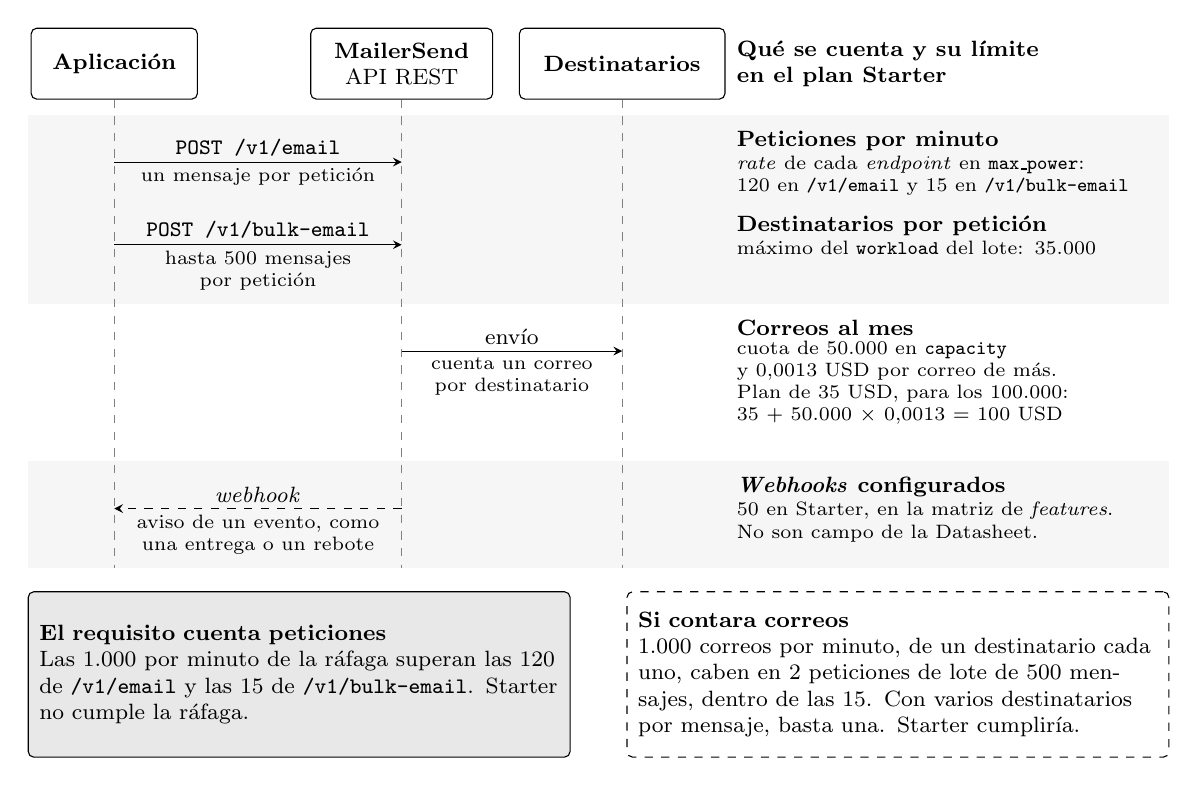
\begin{tikzpicture}[
  font=\footnotesize,
  actor/.style={draw, rounded corners=2pt, align=center, minimum height=9mm, inner sep=3pt},
  cabecera/.style={font=\footnotesize\bfseries, align=left, anchor=west, inner sep=0pt},
  arriba/.style={font=\footnotesize, anchor=south, inner sep=2pt},
  abajo/.style={font=\scriptsize, align=center, anchor=north, inner sep=2pt},
  unidad/.style={font=\footnotesize\bfseries, align=left, text width=55mm, anchor=north west, inner sep=0pt},
  limite/.style={font=\scriptsize, align=left, text width=55mm, anchor=north west, inner xsep=0pt, inner ysep=1.5pt},
  lectura/.style={draw, rounded corners=2pt, align=left, text width=66mm, minimum height=21mm, inner sep=4pt}
]
\fill[gray!7] (0,-1.15) rectangle (14.5,-3.55);
\fill[gray!7] (0,-5.55) rectangle (14.5,-6.9);
\node[actor, text width=19mm] (app) at (1.1,-0.5) {\textbf{Aplicación}};
\node[actor, text width=21mm] (api) at (4.75,-0.5) {\textbf{MailerSend}\\ API REST};
\node[actor, text width=24mm] (dest) at (7.55,-0.5) {\textbf{Destinatarios}};
\node[cabecera, text width=55mm] at (9.0,-0.5) {Qué se cuenta y su límite\\ en el plan Starter};
\draw[dashed, gray] (app.south) -- (1.1,-6.9);
\draw[dashed, gray] (api.south) -- (4.75,-6.9);
\draw[dashed, gray] (dest.south) -- (7.55,-6.9);
\draw[-stealth] (1.1,-1.75) -- node[arriba] {\texttt{POST /v1/email}} node[abajo] {un mensaje por petición} (4.75,-1.75);
\draw[-stealth] (1.1,-2.8) -- node[arriba] {\texttt{POST /v1/bulk-email}} node[abajo] {hasta 500 mensajes\\ por petición} (4.75,-2.8);
\node[unidad] (u1) at (9.0,-1.35) {Peticiones por minuto};
\node[limite] (l1) at (u1.south west) {\textit{rate} de cada \textit{endpoint} en \texttt{max\_power}:\\ 120 en \texttt{/v1/email} y 15 en \texttt{/v1/bulk-email}};
\node[unidad] (u2) at ([yshift=-2mm]l1.south west) {Destinatarios por petición};
\node[limite] at (u2.south west) {máximo del \texttt{workload} del lote: 35.000};
\draw[-stealth] (4.75,-4.15) -- node[arriba] {envío} node[abajo] {cuenta un correo\\ por destinatario} (7.55,-4.15);
\node[unidad] (u3) at (9.0,-3.75) {Correos al mes};
\node[limite] at (u3.south west) {cuota de 50.000 en \texttt{capacity}\\ y 0,0013 USD por correo de más.\\ Plan de 35 USD, para los 100.000:\\ 35 + 50.000 $\times$ 0,0013 = 100 USD};
\draw[-stealth, dashed] (4.75,-6.15) -- node[arriba] {\textit{webhook}} node[abajo] {aviso de un evento, como\\ una entrega o un rebote} (1.1,-6.15);
\node[unidad] (u4) at (9.0,-5.75) {\textit{Webhooks} configurados};
\node[limite] at (u4.south west) {50 en Starter, en la matriz de \textit{features}.\\ No son campo de la Datasheet.};
\node[lectura, fill=gray!18, anchor=north west] at (0,-7.2) {\textbf{El requisito cuenta peticiones}\\ Las 1.000 por minuto de la ráfaga superan las 120 de \texttt{/v1/email} y las 15 de \texttt{/v1/bulk-email}. Starter no cumple la ráfaga.};
\node[lectura, dashed, anchor=north east] at (14.5,-7.2) {\textbf{Si contara correos}\\ 1.000 correos por minuto, de un destinatario cada uno, caben en 2 peticiones de lote de 500 mensajes, dentro de las 15. Con varios destinatarios por mensaje, basta una. Starter cumpliría.};
\end{tikzpicture}
\endgroup

\caption[Conteo del caso de los 100.000 correos en el plan Starter de MailerSend]{Secuencia del caso de los 100.000 correos con el plan Starter de MailerSend, el de su fila en la Tabla~\ref{tab:comparacion:caso}, y lo que cuenta cada paso. Las dos peticiones de envío gastan el \textit{rate} de su \textit{endpoint}, en peticiones por minuto, y la de lote admite además un máximo publicado de 35.000 destinatarios por petición. El envío gasta la cuota mensual, en correos. Los \textit{webhooks} configurados tienen un límite de recursos del plan, no de consumo, que se lee en la matriz de \textit{features}, fuera de la Datasheet. MailerSend no publica en qué unidad cuenta la cuota, y la Datasheet cuenta un correo por destinatario, la unidad con la que el proveedor suma los 35.000 del lote. Abajo, las dos lecturas del requisito de ráfaga, en peticiones y en correos. Elaboración propia a partir de la Datasheet y la matriz de \textit{features} de MailerSend \citep{mailersendpricing,mailersenddocs,mailersendemailapi,mailersendbulk}.}
\label{fig:comparacion:caso}
\end{figure}

Amazon SES no cumple el caso.
SES cobra por destinatario, a 0,10 USD por millar en la tarifa sin suscripción, unos 10 USD para 100.000 correos, pero ese precio está en una nota del \textit{provenance} porque v0.3 no tiene un precio por unidad sin cuota.
Su \textit{rate} en producción no está publicado, y SES no ofrece \textit{webhooks}, porque entrega los eventos de envío a servicios de AWS como Amazon SNS o EventBridge.
El cliente puede recibirlos por HTTP con una suscripción de Amazon SNS, pero el caso solo cuenta como \textit{webhook} el aviso que el propio servicio de correo envía a una URL del cliente, sin otro servicio intermedio.

Mailchimp Transactional queda sin respuesta, porque no publica el caudal de la cuenta de pago y sin él no se puede comprobar la ráfaga.
Sus 100.000 correos son cuatro bloques de 25.000 a 20 USD, 80 USD, con el precio del bloque en ámbar.
El servicio exige además una cuenta de Mailchimp de pago, que la Datasheet no cifra.

El importe de la respuesta depende de los volúmenes contratados: el proveedor vende varios por plan, en la página de precios o en el panel, y la cuota de v0.3 solo admite uno (P-01, Sección~\ref{subsec:evolucion:p01}).
Cada Datasheet modela el volumen mínimo de cada plan, y los demás volúmenes quedan en notas del \textit{provenance}.\footnote{Notas de \texttt{metadata.data\_provenance} en \texttt{03\_datos/apis/<api>/datasheet.yaml} del repositorio del trabajo, con la página de precios o el panel de los que se copiaron.}
SendGrid vende Essentials con 100.000 correos a 34,95 USD, y Resend vende Pro con 100.000 correos a 35 USD.
Mailgun vende Foundation con 100.000 correos a 75 USD.
Postmark vende Basic con 125.000 correos a 115 USD, aunque su panel no declara \textit{webhooks} de eventos para ese plan.

PRIME4API toma de cada plan el único volumen que guarda la cuota, el mínimo, y cobra como sobrecoste lo que pase de él.
Si se usan los volúmenes del \textit{provenance}, Mailgun baja de 90 USD con Scale a 75 con Foundation, y Brevo de 499 USD con Professional a 82 con Starter de 100.000 correos.
Foundation y Starter tienen el mismo \textit{rate}, el mismo lote y los mismos \textit{webhooks} que Scale y Professional, así que también cumplen.

SendGrid sigue siendo la más barata, a 34,95 USD con Essentials 100K, y los 84,95 USD que dan los campos son 2,4 veces el precio que publica para ese volumen.
Con la cuota extendida que propone P-01, una lista de volúmenes con su precio y su sobrecoste, los 34,95 USD de SendGrid, los 75 de Mailgun y los 82 de Brevo saldrían de los campos.

En SendGrid Essentials 50K, el plan que gana el caso cuando solo se leen los campos, la Tabla~\ref{tab:a06-presupuesto} da el tiempo mínimo para 100.000 correos con un destinatario por petición.
Sin sobrecoste son 30 días y 4 segundos, porque los otros 50.000 esperan a que la cuota se reponga, y con un presupuesto que lo cubra son 9 segundos.
Las 16,7 peticiones por segundo del caso son la seiscentésima parte del \textit{rate} que SendGrid publica, y a ese ritmo los 100.000 correos salen en unos 100 minutos, así que en este caso deciden la cuota y el presupuesto.
La curva de capacidad de ese plan (Figura~\ref{fig:capacidad}) se queda en su cuota de 50.000 y no suma el sobrecoste, y una curva para el caso exigiría una ejecución nueva de PRIME4API \citep{prime4apirepo}.

Los \textit{rates} con los que se decide la ráfaga no tienen la misma fiabilidad.
El de SendGrid es una cifra de sus preguntas frecuentes que ninguna cabecera de la respuesta de envío deja ver (Sección~\ref{sec:limites:catalogo}, sobre la procedencia de cada \textit{rate}).
Los de Mailgun, Postmark y Brevo están en ámbar.
El estado de la cuenta también puede bajar el caudal sin cambiar de plan: en MailerSend pasa de 120 a 10 peticiones por minuto con la cuenta en revisión (P-06, el caudal que depende del estado de la cuenta, Sección~\ref{subsec:evolucion:p06}).

El catálogo da veredicto para siete de las ocho APIs, aunque el precio más bajo sale de las notas del \textit{provenance} y los \textit{webhooks}, de la matriz de \textit{features}, que queda fuera del esquema.

\section{Comparación funcional}\label{sec:comparacion:funcional}\label{subsec:hallazgos:funcional}

El catálogo tiene tres preguntas sobre funcionalidades: si el plan gratuito incluye \textit{webhooks}, qué API da IP dedicada (una dirección IP de envío que usa un solo cliente) al menor precio y cuánto tiempo se conservan los registros de envío.
Ninguna se responde con la Datasheet ni con PRIME4API, aunque casi todos los datos que piden están publicados en la página de precios o en el panel de cada API.

Para responderlas se lee la matriz de \textit{features} por plan, una tabla que el ciclo de cada Datasheet rellena con las mismas fuentes (Sección~\ref{sec:propuesta:ciclo}).
Cada celda lleva su cita y su peldaño de la escalera de validación, como el contraste documental o la observación de panel, igual que un campo de la Datasheet, y queda vacía cuando ninguna fuente da el dato.
Ocho de sus filas se registran en las ocho APIs, entre ellas los \textit{webhooks} de eventos, la IP dedicada y la retención de actividad.\footnote{Las ocho matrices, con el literal y la fuente de cada celda, están en \texttt{03\_datos/\allowbreak apis/\allowbreak<api>/\allowbreak features.md} del repositorio de datos del trabajo, \url{https://github.com/danvelcam/tfm-pricing-apis-correo}.}

\subsection{\textit{Webhooks} en el plan gratuito}

PI-E01 pregunta si el plan gratuito incluye \textit{webhooks} de eventos, es decir, avisos HTTP que el proveedor envía cuando un correo se entrega, rebota o se abre.
Como en el caso de los 100.000 correos (Sección~\ref{sec:comparacion:caso}), cuenta como \textit{webhook} el aviso HTTP que el propio servicio de correo envía a una URL del cliente, sin otro servicio intermedio.
Es de clase L, la que se responde leyendo la matriz, y las ocho APIs la contestan.

Cinco de las ocho APIs dan \textit{webhooks} en su plan gratuito o en su cuenta de prueba.
Resend Free y MailerSend Free dan un \textit{webhook} cada uno, y la cuenta de prueba de SendGrid da un \textit{Event Webhook}.
Mailgun los incluye en sus cuatro planes, hasta tres URL por tipo de evento, sin recorte en el plan gratuito.
En Postmark la respuesta es «no consta», porque el panel solo los declara en Pro y Platform.
En Brevo la matriz separa dos cosas: los \textit{webhooks} salientes están en los cinco planes, y los de entrada, que reciben en Brevo eventos de otros sistemas, solo en Professional y Enterprise.

Las dos respuestas atípicas son de las APIs que no tienen un plan gratuito con nombre.
SES no tiene \textit{webhooks} en ningún plan, porque sus eventos salen por otros servicios de AWS, como SNS o EventBridge.
En Mailchimp Transactional la cuenta de prueba no los muestra en el panel y la matriz responde «no consta», aunque la documentación da la operación \texttt{webhooks/add} para la cuenta de pago.

\subsection{IP dedicada al menor precio}

PI-E02 pregunta qué API da IP dedicada al menor precio para 200.000 correos al mes.
Combina un dato de la matriz, la IP dedicada, con el precio de enviar 200.000 correos, que la Datasheet da en todas las APIs salvo SES, y la suma se hace a mano.
SES es la más barata, con 44,95 USD: 20,00 de envío, a 0,0001 USD por destinatario, más 24,95 de una IP estándar.
SES vende la IP sin exigir un volumen mínimo de envío.

Tras SES van Mailgun, con 185 USD (plan Foundation de 100.000 correos a 75, con la IP incluida, más 100.000 de sobrecoste a 1,10 USD el millar), y Mailchimp Transactional, con 189,95 USD (ocho bloques de 25.000 correos a 20 USD más 29,95 de la IP).
Resend cuesta 190 USD (plan Scale de 200.000 correos a 160 más 30 de la IP) y SendGrid 199,95 (plan Pro de 100.000 correos a 89,95, con la IP incluida, más 100.000 de sobrecoste a 0,0011).
Mailchimp adelanta a Resend por cinco céntimos.

Brevo tiene la IP dedicada más barata, 251 USD al año, unos 20,92 al mes, pero solo la vende en el plan Professional.
Ese plan arranca en 150.000 correos por 499 USD, y el volumen contratado que cubre 200.000 es el de 250.000, a 599 USD, así que el coste total queda en unos 620 USD al mes.
Es el coste total más alto de las seis APIs que venden la IP con precio publicado, más del triple que Resend.

Dos APIs quedan fuera de la comparación.
Postmark no es elegible, porque exige 300.000 correos al mes para vender la IP.
MailerSend tampoco, porque su página de precios reserva la IP al plan Enterprise sin publicar su precio.

Dos de las tres cifras más bajas llevan salvedad.
La de Mailchimp Transactional no incluye la cuenta Mailchimp de pago que el producto exige, y con los 25 correos por hora de la cuenta de prueba los 200.000 correos tardarían 333 días.
La de SES no sale de la Datasheet, que no tiene campo para el precio por destinatario, y su entorno de pruebas solo permite 200 correos al día.

\subsection{Retención de la actividad}

PI-E03 pregunta cuánto tiempo conserva cada API los registros de envío, y es de clase X: pide un campo que ACM2YAML v0.3 no tiene.
La matriz tiene valor para siete de las ocho APIs.
Postmark guarda 45 días y Resend 30.
SendGrid guarda entre 3 y 7 días según el plan, y MailerSend entre 1 y 30.
Mailgun guarda los registros entre 1 y 30 días y Mailchimp Transactional 30 días en la cuenta de prueba.
En Brevo el periodo lo fija el cliente entre 1 y 24 meses, y es el único caso de las ocho APIs en que no lo pone el proveedor.
En SES ninguna fuente publica la retención, así que la pregunta no tiene respuesta en ningún sitio.

La pregunta sigue en clase X aunque la matriz tenga siete valores, porque la retención es un límite de uso, el máximo de un nivel de uso medible, y no una \textit{feature}.
A diferencia de la cuota mensual, no se gasta con cada envío, y ACM2YAML v0.3 no tiene campo para ese tipo de límite.

\subsection{Lo que la matriz añade}

Con la matriz el catálogo pasa de 25 a 27 preguntas respondibles, porque se suman las dos de clase L.
Las ocho APIs ganan dos respuestas cada una y quedan entre las 20 de Postmark y las 24 de Resend.
Las preguntas comunes a las ocho APIs pasan de 16 a 18, porque se añaden las dos de clase L, PI-E01 y PI-E02.

El resultado deja una asimetría entre los dos tipos de pregunta.
La capacidad se responde con instrumento, ya sea leyendo campos de la Datasheet o ejecutando PRIME4API, mientras que las \textit{features} se responden leyendo la matriz a mano.
En PI-E02 la IP dedicada de cada API está en la matriz y el precio de los 200.000 correos, en la Datasheet salvo en SES, y ninguna herramienta une las dos mitades.
Lo que haría a PI-E02 respondible con instrumento es un vínculo entre la Datasheet del canal API y el iPricing, el metamodelo con el que SPHERE representa los planes y las \textit{features} que un SaaS publica en su canal web \citep{garciafernandez2024pricing4saas}.
Ese vínculo cae fuera del alcance fijado en el Capítulo~\ref{cap:catalogo}, que modela solo el canal API, y por eso la comparación funcional se queda en lectura trazada, celda a celda, sin cálculo automático.

\section{Respuesta a la RQ4}
\label{sec:comparacion:respuesta}

La RQ4 pregunta cómo pueden compararse las APIs de correo de forma sistemática para responder a preguntas de decisión que involucran simultáneamente requisitos funcionales y no funcionales.
La respuesta es un procedimiento que instancia cada una de las 32 plantillas del catálogo sobre cada API.
Cada instancia se responde con el instrumento que declara su clase: un campo de la Datasheet, una operación de PRIME4API, una composición de HARVEY4API o la matriz de \textit{features} por plan.
Cada respuesta queda registrada con la fuente que la sostiene.

Con ese instrumental, 25 de las 32 preguntas tienen una clase que las declara respondibles con la Datasheet, PRIME4API o HARVEY4API.
Si se descuentan las cuatro de HARVEY4API, que no se ha ejecutado, quedan 21.
Otras 2, fuera de esas 25, se responden leyendo la matriz de \textit{features}.
Las cinco restantes señalan lo que falta, como la concurrencia de peticiones, que ACM2YAML v0.3 no serializa, o la retención de los registros de envío, un límite que no se gasta con cada envío.

Cada API responde entre 18 de esas 25 preguntas, en Postmark, y 22, en Resend (Tabla~\ref{tab:cobertura-pi}).
En SES, 17 de sus 21 respuestas no se dan sobre el plan de suscripción que presupone la pregunta: 16 se dan sobre el entorno de pruebas y una sobre la tarifa sin suscripción.
En Mailchimp, 10 de 20 son de la cuenta de prueba.

La comparación es asimétrica.
El coste, la cuota y el caudal se comparan calculando sobre la Datasheet con PRIME4API, y los \textit{webhooks} o la IP dedicada se comparan leyendo a mano la matriz de \textit{features}.
El caso de los 100.000 correos al mes necesita las dos: el precio, el caudal y el lote salen de la Datasheet, y los \textit{webhooks}, de la matriz.
Cumplen SendGrid, Mailgun, Postmark y Brevo, y la más barata es SendGrid, a 34,95 USD al mes con Essentials 100K.
Con los campos de v0.3 saldría a 84,95 USD, 2,4 veces el precio que SendGrid publica para ese volumen, porque la cuota no guarda el volumen de 100.000 correos (Sección~\ref{sec:comparacion:caso}).

La respuesta tiene dos límites.
La base son ocho APIs, y en cinco de ellas lo observado con cuenta propia corresponde a un estado de la suscripción, la fase en que el proveedor sitúa la cuenta, y no a un plan.
Son el entorno de pruebas en SES, la cuenta de prueba en Mailchimp y una cuenta gratuita o sin aprobar en MailerSend, Mailgun y Brevo.
El segundo límite es que las cuatro preguntas que combinan varias Datasheets o varias operaciones cuentan como respondibles por la especificación de HARVEY4API que publica Ruiz López \citep{ruizlopez2026tfm}, sin que la herramienta se haya ejecutado.
Las respuestas que dio Claude Opus 5.5 leyendo las ocho Datasheets llegan a la misma conclusión que la referencia calculada a mano, pero no sustituyen a la herramienta (Sección~\ref{sec:comparacion:harvey}).

